% Chapter Template

\chapter{Results} % Main chapter title
\label{chap:results} % Change X to a consecutive number; for referencing this chapter elsewhere, use \ref{ChapterX}
This chapter will summarize the results of this work. First, the results of simulating the susceptible population
in the region of Hesse will be presented. Then the results of a sensitivity analysis for the variables $\alpha$ and
$q$ will be shown. Specifically the sensitivity analysis will later be used in \hyperref[chap:discussion]{Chapter
\ref*{chap:discussion} - Discussion} to explain the results of the simulations.


%----------------------------------------------------------------------------------------
%	SECTION 1
%----------------------------------------------------------------------------------------

\section{Simulating the susceptible population of Hesse}
During this work we simulated the susceptible population of Hesse. 26 regions were simulated over a time period of
76, 60 and 50 days respectively. We will present both the absolute and percentage difference between the simulated
and the original data for each time frame.

%-----------------------------------
%	SUBSECTION 1
%-----------------------------------
\subsection{Simulating susceptibles in a 76 day time frame}
We first wanted to observe how well the simulation performs in a time frame of 76 days. Since the number of susceptible
individuals is much greater then any other group at any given data point, changes in this group can be difficult to
observe. Because of this we decided to calculate and compare the number of individuals that migrated from the susceptible
to the exposed group instead. This was done by subtracting the number of susceptible individuals at data point \I{t=x} from
the start point \I{t=0}. The result is the total change of susceptibles at any given time point, which is equivalent to the 
sum of all exposed individuals at any given time point. These results are much easier to compare and understand.
\hyperref[fig:76_sim_expl]{figure \ref*{fig:76_sim_expl}} shows three graphs that illustrate this process.


\begin{figure}
	\centering
	\begin{subfigure}[b]{0.3\textwidth}
		\centering
		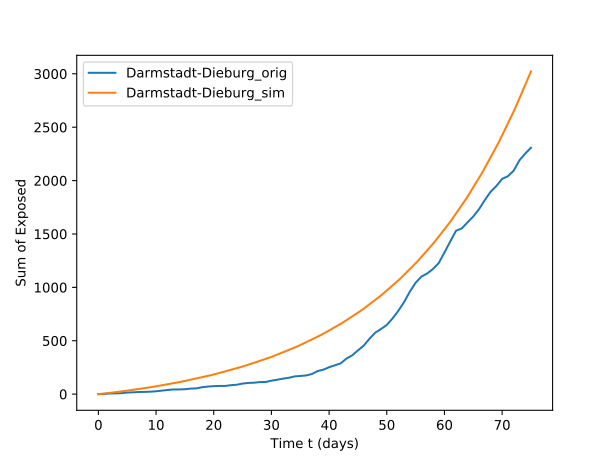
\includegraphics[width=\textwidth]{./figures/24_Darmstadt-Dieburg.png}	
		\caption{}
	\end{subfigure}
	\hfill
	\begin{subfigure}[b]{0.3\textwidth}
		\centering
		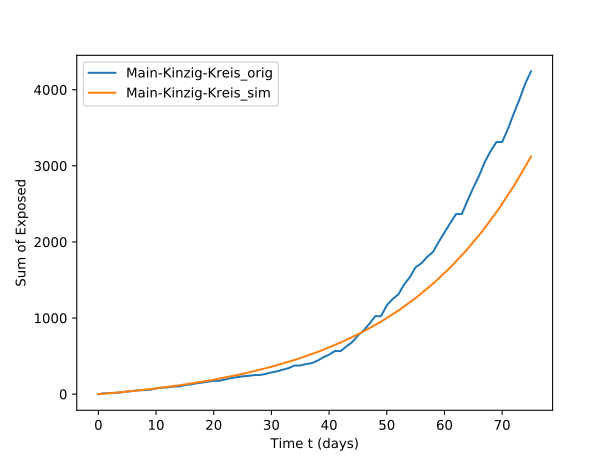
\includegraphics[width=\textwidth]{./figures/13_Main-Kinzig-Kreis.png}	
		\caption{}
	\end{subfigure}
	\hfill
	\begin{subfigure}[b]{0.3\textwidth}
		\centering
		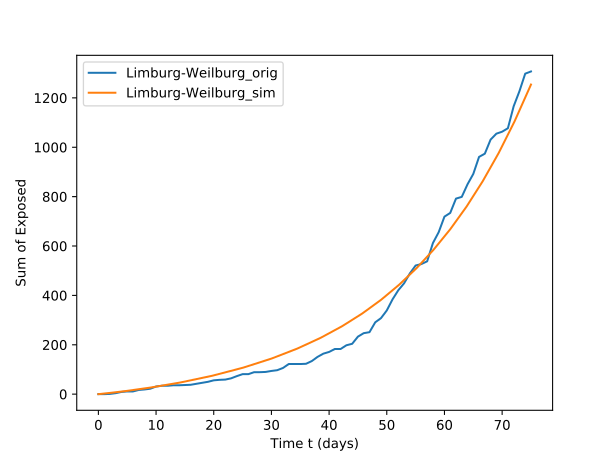
\includegraphics[width=\textwidth]{./figures/10_Limburg-Weilburg.png}	
		\caption{}
	\end{subfigure}
	\caption{Three exemplary results of a simulation of the exposed individuals.
		The original (``orig'') data is drawn in a blue, the simulated (``sim'') data is drawn in an orange line.
		The number of simulated individuals can be greater (image (A), region ``Darmstadt Dieburg''), smaller 
		(image (B), region ``Mein Kinzig Kreis'') or about the same (image (C), region ``Limburg Weilburg''), as 
		the originally observed number of exposed.
		}
	\label{fig:76_sim_expl}
\end{figure}

Furthermore we analyzed the percentage deviation of original and simulated data for each time step in each region. The results
are shown in a box plot in \hyperref[fig:76_sim_box]{figure \ref*{fig:76_sim_box}}. The three regions ``Werra-Meissner-Kreis'',
``Marburg-Biedenkopf'' and ``Limburg-Weilburg'' are listed separately in figure \ref*{fig:76_sim_box}, in order to make the scales
more readable.


\begin{figure}
	\centering
	\begin{subfigure}[b]{0.4\textwidth}
		\centering
		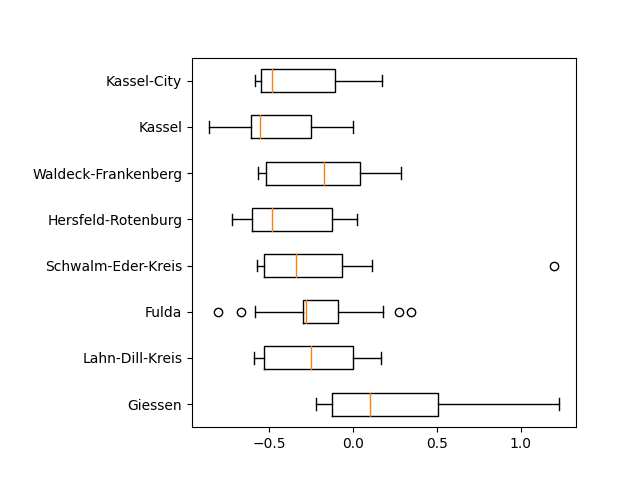
\includegraphics[width=\textwidth]{./figures/deviation_box_alt1.png}	
	\end{subfigure}
	\begin{subfigure}[b]{0.4\textwidth}
		\centering
		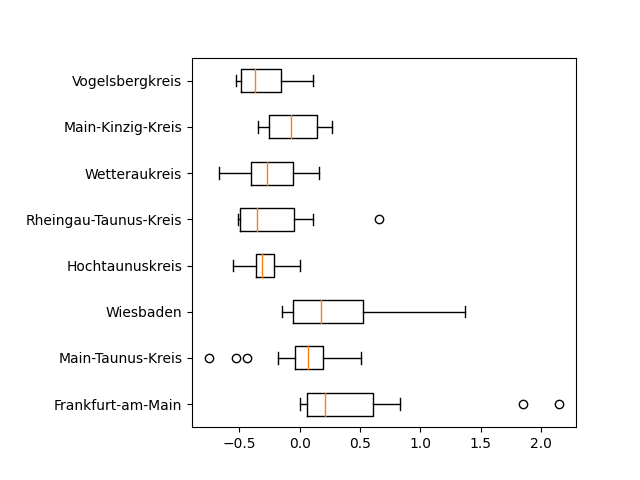
\includegraphics[width=\textwidth]{./figures/deviation_box_alt2.png}	
	\end{subfigure}
	\begin{subfigure}[b]{0.4\textwidth}
		\centering
		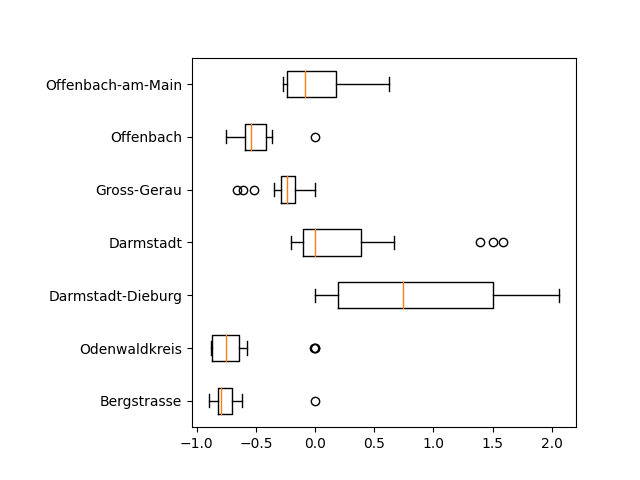
\includegraphics[width=\textwidth]{./figures/deviation_box_alt3.png}	
	\end{subfigure}
	\begin{subfigure}[b]{0.4\textwidth}
		\centering
		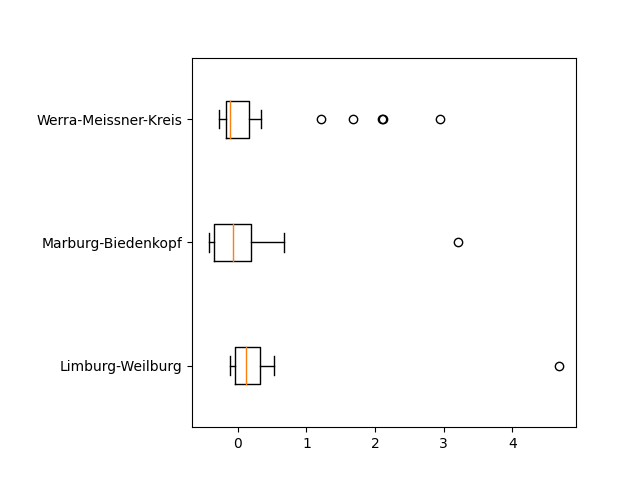
\includegraphics[width=\textwidth]{./figures/deviation_box_alt4.png}	
	\end{subfigure}
	\caption{Shown are box plots of the percentage deviation, of every simulated region relative to the original data.}
	\label{fig:76_sim_box}
\end{figure}

Figure \fred*{fig:76_sim_box} shows that most of the simulated regions show a wide range of median values, ranging between
-100 and +100 percent deviation.



%-----------------------------------
%	SUBSECTION 2
%-----------------------------------
\subsection{Simulating susceptibles in a 60 day time frame}


%-----------------------------------
%	SUBSECTION 2
%-----------------------------------
\subsection{Simulating susceptibles in a 50 day time frame}


%----------------------------------------------------------------------------------------
%	SECTION 2
%----------------------------------------------------------------------------------------

\section{Sensitivity analysis of $\alpha$ and $q$}

